\documentclass[a4paper]{article}
\usepackage[utf8]{inputenc}
\usepackage[T2A]{fontenc}
\usepackage[12pt]{extsizes}
\everymath{\displaystyle}

\usepackage[english,russian]{babel}
\usepackage[left=10mm, top=10mm, right=10mm, bottom=20mm, nohead, nofoot]{geometry}
\usepackage{amsmath,amsfonts,amssymb} % математический пакет
\headsep=10mm

\usepackage{alltt}
\usepackage[most]{tcolorbox} % для управления цветом
% НАСТРОЙКИ
%теорема
\definecolor{theorem-color}{gray}{0.90} % уровень прозрачности (1 - максимум)
\newtcolorbox{htheorem}{colback=theorem-color,grow to right by=-4mm,grow to left by=-4mm,
    boxrule=0pt,boxsep=0pt,breakable} % настройки области с изменённым фоном

%определение
\definecolor{def-color}{gray}{0.98}
\newtcolorbox{definit}{colback=def-color,grow to right by=-4mm,grow to left by=-4mm,
    boxrule=0pt,boxsep=0pt,breakable} % настройки области с изменённым фоном

%доказательсвто теоремы
\definecolor{proof-color}{gray}{0.95} % уровень прозрачности (1 - максимум)
\newtcolorbox{hproof}{colback=proof-color,grow to right by=-1mm,grow to left by=-1mm,
    boxrule=0pt,boxsep=0pt,breakable} % настройки области с изменённым фоном

%замечания, следствия
\definecolor{consectary-color}{gray}{0.95} % уровень прозрачности (1 - максимум)
\newtcolorbox{cns}{colback=consectary-color,grow to right by=-4mm,grow to left by=-4mm,
    boxrule=0pt,boxsep=0pt,breakable} % настройки области с изменённым фоном



\usepackage{fancybox,fancyhdr}
\pagestyle{fancy}

\usepackage{hyperref}
\hypersetup{colorlinks=true, allcolors=[RGB]{010 090 200}} % цвет ссылок 
\newcommand{\lr}[1]{\left({#1}\right)} % команда для скобок

\author{Васильев Павел}
%\linespread{1}
\usepackage{amsmath}

\usepackage{graphicx}
\usepackage{ifpdf}
\ifpdf
\DeclareGraphicsRule{*}{mps}{*}{}
\fi
\usepackage{graphicx}
\usepackage{color}
\graphicspath{ {images/} }


\renewcommand{\headrulewidth}{0pt}

%\renewcommand{\familydefault}{\sfdefault}

\begin{document}

\section*{HOW TO заботать собеседование в Яндекс на ML-стажировку}

\section*{Вопросы к собеседованию}

\subsection*{Линейные модели}

\begin{itemize}

\item \textit{Опишите задачу машинного обучния. Дайте определение объекту, целевой переменной, признакам, модели, функционалу ошибку}.

Объект - то, для чего мы хотим сделать какое-то предсказание. Целевая переменная - величина, которую мы хотим определять. Признаки - это набор характеристик для выборки объектов. Модель машинного обучения - это метод обучения компьютера, который позволяет выявить какие-то закономерности, благодаря которым сможет строить прогнозы целевой переменной. Функционал ошибки - функция, которая принимает на вход ответы алгоритма и правильные ответы и возвращает число, которое характеризует качество обученности модели.

\item \textit{Чем отличается функция потерь от функционала ошибки?}

Ничем.

\item \textit{Какие функции потерь используются при решении задачи регрессии?}

\begin{itemize}
\item \[ MSE(a, X) = \frac{1}{l} \sum_{i=1}^l (a(x_i) - y_i)^2 \]

MSE не сохраняет единицы измерения, например, если предсказывали цену в рублях, то MSE будет показывать рубли в квадрате.

\item \[ RMSE(a, X) = \sqrt{ \frac{1}{l} \sum_{i=1}^l (a(x_i) - y_i)^2 }\]

RMSE подходит для контроля качества во время обучения или для сравнения двух моделей, но не показывает то, насколько хорошо молель решает задачу. Типа если MSE = 100 и правильный ответ маленький по модулю, то эта ошибка слишком большая, а если правильный ответ > 100000, то такая ошибка очень маленькая.

\item Коэффициент детерминации $R^2$:

\[ R^2(a, X) = 1 - \frac{\sum_{i=1}^l (a(x_i) - y_i)^2}{\sum_{i=1}^l (y_i - \overline{y_i})^2}, \overline{y} = \frac{1}{l} \sum_{i=1}^l y_i \]

В числителе стоит дисперсия модели относительно правильных ответов, а в знаменателе общая дисперсия ответов.

Короче, это нормированная среднеквадратическая ошибка. Если эта ошибка близка к единице, это значит, что относительная дисперсия маленькая, значит модель хорошо описывает данные. А если близка к нулю, то модель похожа на константное предсказание.

\item \[ MAE(a, X) = \frac{1}{l} \sum_{i=1}^l |a(x_i) - y_i | \]

Модуль менее чувствителен к выбросам, но недифференцируем.
Но проблема недифференцируемости не сильно плохая (мы можем дополнить производную в точках разрыва какими-нибудь значениями). Основная проблема в том, что при градиентном спуске нам по функции потерь хочется понимать, насколько текущий прогноз модели близок к правильному ответу.

А производная модуля это функция $sign$, ну понятно.

\item HuberLoss:

\[ L_\delta(y, a) = \begin{cases}
\frac{1}{2} (y-a)^2, |y-a| < \delta \\
\delta \left( |y-a| - \frac{1}{2} \delta \right), |y-a| \geq \delta
\end{cases} \]

$\delta$ отвечает за то, что мы считаем за выбросы, а что нет.

\item Log-cosh:

\[ L(y, a) = \log \cosh (a-y) \]

Для маленьких отклонений здесь квадратичное поведение, для больших - линейное.

\item MSLE:

\[ L(y, a) = (log(a+1) - log(y+1))^2 \]

Подходит для задач с неотрицательным таргетом и неотрицательными прогнозами модели. Поскольку мы берём квадрат разностии именно логарифмов, то штрафуем мы за отклонения в порядке величин, а не в их значениях. И кстати, за заниженные прогнозы эта ошибка штрафует сильнее чем за завышенные, потому что логарифм.

\item MAPE, SMAPE

\[ L(y, a) = \left| \frac{y-a}{y} \right| \]

Эта функция ошибки заставляет нас не думать о масштабе данных, потому что мы нормируем по таргету отклонение. Но: если $y=1$ и все прогнозы $\geq 0$, то максимальная ошибка заниженного прогноза $=1$, а завышенного неограничена сверху.

Эту проблему решает SMAPE:

\[ L(y, a) = \frac{|y-a|}{\frac{|y|+|a|}{2}} \]
\end{itemize}

\item \textit{Запишите формулу для линейной модели регрессии}

\[ a(x) = w_0 + w_1 x + ... + w_d x_d \]

\[ a(x) = w_0 + \langle w, x \rangle \]

Ну часто $w_0$ включают в вектор $w$: $w = (w_0, ..., w_d)$, $a(x) = \langle w, x \rangle$ ($d$ - число признаков, $x = (1, x_1, ..., x_d)$ - признаковое описание объекта $x$.

\item \textit{Чем отличаются функционалы MSE и MAE? В каких случаях лучше использовать MSE, а в каких MAE?}

\[ MSE(a, X) = \frac{1}{l} \sum_{i=1}^l (a(x_i) - y_i)^2 \]
\[ MAE(a, X) = \frac{1}{l} \sum_{i=1}^l |a(x_i) - y_i | \]

MSE чувствителен к выбросам в данных, поскольку отклонение вносит вклад квадратично, MAE же просто смотрит на отклонение предсказание от ответа, поэтому он более терпим к выбросам, то есть обучая модель с MAE функцией ошибки, то мы  допускаем выбросы в датасете.

\item \textit{Чем отличается MAE от MAPE? Что более понятно заказчику продукта?}

\[ MAE(a, X) = \frac{1}{l} \sum_{i=1}^l |a(x_i) - y_i | \]
\[ MAPE(a, X) = \left| \frac{y-a}{y} \right| \]

MAPE позволяет работать с данными разного масштаба. При этом MAPE обладает особенностью: допустим у нас $y = 1$ и все прогнозы $\geq 0$, то максимальная ошибка заниженного прогноза равна 1, а завышенного не ограничена сверху.

\item \textit{Что такое коэффициент детерминации? Как интерпретировать его значения?}

\[ R^2(a, X) = 1 - \frac{\sum_{i=1}^l (a(x_i) - y_i)^2}{\sum_{i=1}^l (y_i - \overline{y_i})^2}, \overline{y} = \frac{1}{l} \sum_{i=1}^l y_i \]

Измеряет долю дисперсии, объяснённую моделью, в общей дисперсии таргета. Короче, это нормированная среднеквадратичная ошибка. Если дисперсия нашей модели такая же как и дисперсия таргета, то модель фиговая, а если дисперсия модели относительно дисперсии таргета мала, то модель неплохо предсказывает целевую переменную.

\item \textit{$log-cosh$ лучше функции потерь Хубера? Опишите обе функции потерь.}

Huber-loss:

\[ L_\delta(y, a) = \begin{cases}
\frac{1}{2} (y-a)^2, |y-a| < \delta \\
\delta \left( |y-a| - \frac{1}{2} \delta \right), |y-a| \geq \delta
\end{cases} \]

Log-cosh:

\[ L(y, a) = \log \cosh (a-y) \]

Log-cosh лучше Хубера тем, что у Хубера вторая производная разрывна. В остальном, они обе при маленьких отклонениях ведут себя квадратично, а при больших - линейно.

\item Что такое градиент? Какое его свойство используется при минимизации функций?

Градиент - вектор частных производных. Главное свойство - показывает направление наискорейшего возрастания функции. Находя градиент функции потерь по весам модели и двигаясь в противоположную сторону, мы уменьшаем ошибку.

\item \textit{Что такое градиентный спуск? Опишите процесс алгоритма.}

Градиентный спуск - итерационный алгоритм, который вот в чём заключается:

\begin{itemize}

\item Инициализируем $w^{(0)}$ как-нибудь

\item $w^{(k)} = w^{(k-1)} - \eta_k \nabla Q(w^{(k-1)})$, $\eta_k = \frac{1}{k}$

\end{itemize}

\item  Почему не всегда можно использовать полный градиентный спуск? Какие способы
оценивания градиента вы знаете? Почему в стохастическом градиентном спуске важно
менять длину шага по мере итераций? Какие стратегии изменения шага вы знаете?

Градиентный спуск не всегда можно использовать банально потому, что функция ошибки может быть недиферренцируемой.
Ещё это может быть связано с тем, что в некоторых местах функция ошибки близка к константе, и если в процессе градиентного спуска прийти в эту область, то он будет очень долго сходиться. Также градиентный спуск может не сойтись, если у нас сложная поверхность функции ошибки - несколько локальных минимумов.

Вот еще условия сходимости градиентного спуска: функция выпуклая и дифференцируемая, первая производная является липшицевой.

Полный град. спуск лучше не использовать, если объектов очень и очень много - он просто считаться долго будет.

Оценивание градиента:
как правило, функция ошибки представима в виде суммы ошибок на всех объектах:

\[ Q(w) = \frac{1}{l} \sum_{i=1}^l q_i(w) \]

Но можно не брать всю сумму, так как при большой выборке это слишком трудоёмкая операция, а можно оценивать весь градиент градиентом одного случайного объекта:

$\nabla_w Q(w) \approx \nabla_w q_{i_k} (w)$

$w^{(k)} = w^{(k-1)} - \eta_k \nabla q_{i_k} ( w^{(k-1)} ) $

Так как мы весь градиент оцениваем градиентом на одном объекте, то он может не замедляться вблизи точки минимума, так как параметры, оптимальные для всех объектов, могут не совпадать с параметрами для выбранного объекта. Поэтому необходимо самим уменьшать шаг стохастического градиентного спуска.

Шаг $\eta_k$ можно выбирать разным, главное, чтобы он удовлетворял условиям Роббинса-Монро:

\[ \sum_{k=1}^\infty \eta_k = \infty, \sum_{k=1}^\infty \eta_k^2 < \infty \]

Можно брать $\eta_k = \frac{1}{k}$, а можно $\eta_k = \lambda \left( \frac{s_0}{s_0+k} \right) ^k$, где $\lambda, s_0, p$ - параметры, $s_0 = 1, p = 0.5, d = 1$, $\lambda$ настраивается.

\item Что такое метод среднего стохастического градиента? В чём его плюсы относительно полного и стохастического градиентного спуска?

Метод заключается в следующем:

\begin{itemize}

\item Инициализируем как-нибудь $w^{(0)}$
\item Берём вспомогательную переменную $z_i^{(0)} = \nabla q_i (w^{(0)}), i = 1, ..., l$
\item На $k$-ой итерации берём случайный индекс $i_k$ и выполняем $z_i^{(k)} = \begin{cases}
\nabla q_i (w^{(k-1)}), if i = i_k \\
z_i^{(k-1)} else
\end{cases} $

\end{itemize}

И тогда $\nabla_w Q(w) \approx \frac{1}{l} \sum_{i=1}^l x_i^{(k)}$.

В этом методе мы обязаны хранить последние вычисленные градиенты для всех объектов выборки.

$w^{(k)} = w^{(k-1)} - \eta_k \sum_{i=1}^l z_i^{(k)}$


\item Какие модификации градиентного спуска еще есть?

\begin{itemize}

\item \textbf{Метод инерции (momentum).}

Если в обычном градиентном спуске у нас градиент сильно меняет направление от шага к шагу, то стоит его усреднить последними шагами. Для этого вводится 
\[ h_0 = 0 \]

\[ h_k = \alpha h_{k-1} + \eta_k \nabla_w Q(w^{(k-1)})\]

$\alpha$ отвечает за вклад градиентов с предыдущих шагов.

\item \textbf{AdaGrad, RMSprop.}

В методе AdaGrad предлагают сделать свою длину шага для каждой компоненты вектора параметров:

\[ G_{kj} = G_{k-1, j} + \left( \nabla_w Q(w^{(k-1)} ) \right)_j^2 \]

\[ w_j^{(k)} = w_j^{(k-1)} - \frac{\eta_t}{\sqrt{G_{kj}+\varepsilon}} \left( \nabla_w Q(w^{(k-1)}) \right)_j \]

\[ G_{k} = G_{k-1} + \left( \nabla_w Q(w^{(k-1)} ) \right)^2 \]

\[ w^{(k)} = w^{(k-1)} - \frac{\eta_t}{\sqrt{G_{k}+\varepsilon}} \left( \nabla_w Q(w^{(k-1)}) \right) \]


$\varepsilon$ нужен, чтобы корешок в ноль не превратился

Идея следующая: если мы вышли на плато по какой-то координате и соответствующая компонента градиента начала затухать, то нам нельзя уменьшать размер шага слишком сильно, так как мы рискуем на этом плато остаться, но в то же время уменьшать надо, потому что это плато может содержать оптимум. Если же градиент долгое время большой, то это может быть знаком, что нам нужно уменьшить размер шага, чтобы не пропустить оптимум. Поэтому мы стараемся компенсировать слишком большие или слишком маленькие координаты градиента.

Заметим, что $G_{kj}$ растёт, поэтому, шаги становятся всё медленнее, и градиентный спуск может остановиться раньше, чем нужно.

RMSprop использует экспоненциальное затухание градиентов:

\[ G_{kj} = \alpha G_{k-1,j} + (1-\alpha) \left( \nabla_w Q( w^{(k-1)}) \right)_j^2 \]

Тут уже размер шага по координате зависит от того, насколько быстро мы двигались по ней на последних шагах.

\item \textbf{Adam} 

Этот метод совмещает Momentum и AdaGrad (RMSprop):

\[ h_k = \beta_1 h_{k-1} + (1-\beta_1) \nabla_w Q( w^{(k-1)} )\]

\[ G_{k+1} = \beta_2 G_k + (1-\beta_2) \left( \nabla_w Q(w^{(k-1)}) \right)^2 \]

\[ w^{(k)} = w^{(k-1)} - \frac{\alpha}{\sqrt{(G_{k+1} + \varepsilon)}} h_{k-1}\]

\item \textbf{AdamW}

Добавим к Adam $l_2$ регуляризацию

\end{itemize}


\item \textit{Что такое переобучение? Как можно отследить переобучение модели?}

Переобучение - это состояние модели, когда на тренировочной выборке она показывает очень высокое качество, а на тестовой непозволительно низкое.

Как правило, когда модель переобученаа, мы можем посмотреть на её веса, и они оказываются большими по модулю. Фактически, это значит, что модель излишне подстроилась под обучющую выборку. Например, если у нас было несколько выбросов, то в линейной модели будут большие коэффициенты.

Также можно заметить переобучение с помощью валидационной выборки и кросс-валидации.

\item \textit{Что такое кросс-валидация? На что влияет количество блоков в кросс-валидации?}

Кросс-валидация - метод оценивания качества модели, который заключается в следующем: выборка делится на $k$ фолдов. Для каждого $1\leq i \leq k$ модель обучается на всех фолдах, кроме $i$-ого, а тестируется на $i$-ом. И берётся среднее со всех полученных ошикок. Таким образом, мы как будто увеличиваем размер выборки, и тестируем модель на немного разных входных данных. Вообще, кросс-валидация - частный случай бэггинга.

\item \textbf{Как построить итоговую модель после того, как по кросс-валидации подобраны
оптимальные гиперпараметры?}

\item \textit{Что такое регуляризация? Для чего используется?}

Регуляризация - способ борьбы с переобучением модели. Переобучение часто приводит к большим коэффициентам. Чтобы этого избежать, добавим ещё штраф за норму вектор весов:

\[ Q_\alpha (w) = Q(w) + \alpha R(w)\]

\[ R(w) = |w|_2 = \sum_{i=1}^d w_i^2 \]

\[ R(w) = |w|_1 = \sum_{i=1}^d |w_i| \]

Тут надо отметить, что $w_0$ регуляризовывать не надо, так как этот вес не связан с признаками объектов, он отвечает лишь за смещение модели.

\item \textit{Опишите, как работают L1- и L2-регуляризаторы.}

$L_1$ регуляризатор зануляет незначимые признаки. Это происходит потому, что если на плоскости с осями двух каких-то весов модели изобразить $|w|_1$, то она будет лежать внутри квадрата. Фукнция ошибки имеет эллипсовидные линии уровня, и вероятность того, что линия уровня (которая соответствует достаточно низкому значению функции ошибки) пройдёт через "угол" квадрата повыше, чем если линия уровня пересечёт квадрат где-то по-середине. А в углу квадрата одна из компонент вектора $w$ занулена. У $L_2$ регуляризации такого прикола нет, потому что норма ограничена окружностью, и там таких углов, как у квадрата, нет.
Ещё при $L_2$ регуляризации меньше шансов, что маленькие веса будут окончательно обнулены.

\item \textbf{Где используется метод максимального праводоподобия?}

\item \textit{Расскажите про метрики, которые штрафуют за перепрогноз сильнее, чем за
недопрогноз и наоборот(pinball loss)
}

MSLE:
\[ L(y, a) = (log(a+1) - log(y+1))^2 \]

Подходит для задач с неотрицательным таргетом и неотрицательными прогнозами модели. Поскольку мы берём квадрат разностии именно логарифмов, то штрафуем мы за отклонения в порядке величин, а не в их значениях. И кстати, за заниженные прогнозы эта ошибка штрафует сильнее чем за завышенные, потому что логарифм.

\item \textit{Расскажите про виды скейлинга. Зачем они нужны?}

Если не масштабировать данные, то в антиградиенте некоторые компоненты могут быть огромные, из-за чего спуск будет ковылять вокруг минимума, но не попадёт в него, потому что будет всё время перескакивать его. Можно даже уйти от минимума при неправильном подборе длины шага.

Масштабировать можно так:

\[ x_{ij} := \frac{x_{ij} - \mu_j}{\sigma_j}, \mu_j = \mathbb{E} x_{ij}, \sigma_j = \mathbb{D} x_{ij} \]

или так 

\[ x_{ij} := \frac{x_{ij} - \min_i x_{ij}}{max_i x_{ij} - min_i x_{ij}} \]

\item \textit{Как записываются аналитическое решения? Какие у них проблемы?}

\begin{equation}
\begin{gathered}
Loss = \frac{1}{n} (Xw -y)^T (Xw - y) = \\
= \{ a = Xw - y \} = \frac{1}{n} a^T a \\
\frac{\partial Loss}{\partial w} = \left( \frac{\partial a^T}{\partial w} a + a^T \frac{\partial a}{\partial w} \right) \frac{1}{n} = \\
= \frac{1}{n} \left( a^T \left( \left( \frac{\partial a}{\partial w} \right)^T \right)^T + a^T \frac{\partial a}{\partial w} \right) =  \\
= \frac{2}{n} \left( a^T \frac{\partial a}{\partial w} \right) = \frac{2}{n} a^T X = \frac{2}{n} \left( Xw-y \right)^T X = \frac{2}{n} \left( w^TX^TX-y^TX \right) = 0\\
w^T = y^TX (XTX)^{-1} \\
w = \left( y^TX (X^TX)^{-1} \right)^T\\
w = (X^TX)^{-1}X^Ty
\end{gathered}
\end{equation}

Проблемы: обращение матрицы - неустойчивая операция,

\end{itemize}


\subsection*{Классификация}

\begin{itemize}

\item \textit{Запишите формулу для линейной модели классификации. Что такое отступ?}

$\mathbb{Y} = \{ -1, 1 \}$

\[ a(x) = sgn \langle w, x \rangle \]

Ой, а если $\langle w, x \rangle = 0$?

Можем поступить так:
\begin{itemize}
\item Сказать, что такого никогда не бывает
\item Отказаться от классификации
\end{itemize}

Отступ:

\[ M_i = y_i \langle w, x_i \rangle \]

Знак отступка отражает корректность ответа классификатора, а его абсолютное значение - уверенность модели в своём ответе.

\item \textit{Как обучаются линейные классификаторы и для чего нужны верхние оценки пороговой функции потерь?}

Очевидным функционалом качества служит доля правильных ответов, тогда функция ошибки такая:

\[  Q(a, X) = \frac{1}{l} \sum_{i=1}^l [a(x_i) \neq y_i] \rightarrow \min_w \]

\[ Q(a, X) = \frac{1}{l} \sum_{i=1}^l [y_i \langle w, x \rangle < 0] \rightarrow \min_w \]

Эта функция некрасивая - она разрывная, градиентным спуском по ней не походишь - она всюду константа, кроме как в нуле. Поэтому придумали верхние оценки:

\begin{itemize}
\item $ \widetilde{L}(M) = \log (1+e^{-M} $ - логистическая
\item $ \widetilde{L}(M) = \max(0, 1-M)$
\item $ \widetilde{L}(M) = e^{-M}$ - экспоненциальная
\item $ \widetilde{L}(M) = \frac{2}{1+e^M}$ - сигмоидная
\end{itemize}

\item \textit{Что такое точность, полнота и F-мера? Почему F-мера лучше арифметического среднего и минимума?}

Точность (precision) - показывает, какая доля объектов, выделенных классификатором как положительные, реально положительные.

Полнота (recall) - показывает, какая часть положительных объектов была выделена классификатором.

\[ precision = \frac{TP}{TP+FP} \]

\[ recall = \frac{TP}{TP+FN} \]

Это две метрики, хотим оптимизировать одну.

Допустим берём среднее арифметическое. Тогда модель с ужасным precision и большим recall покажет такую же метрику как модель с средненьким precision и recall. Так не пойдёт.

Допустим берём минимум. Тогда считается, что если recall больше чем precision, то модели с равным recall и любым precision будут считаться одинаковыми по качеству, но это совсем не так.

F-мера - это сглаженная версия минимума:

\[ F = \frac{2 \cdot precision \cdot recall}{precision + recall} \]

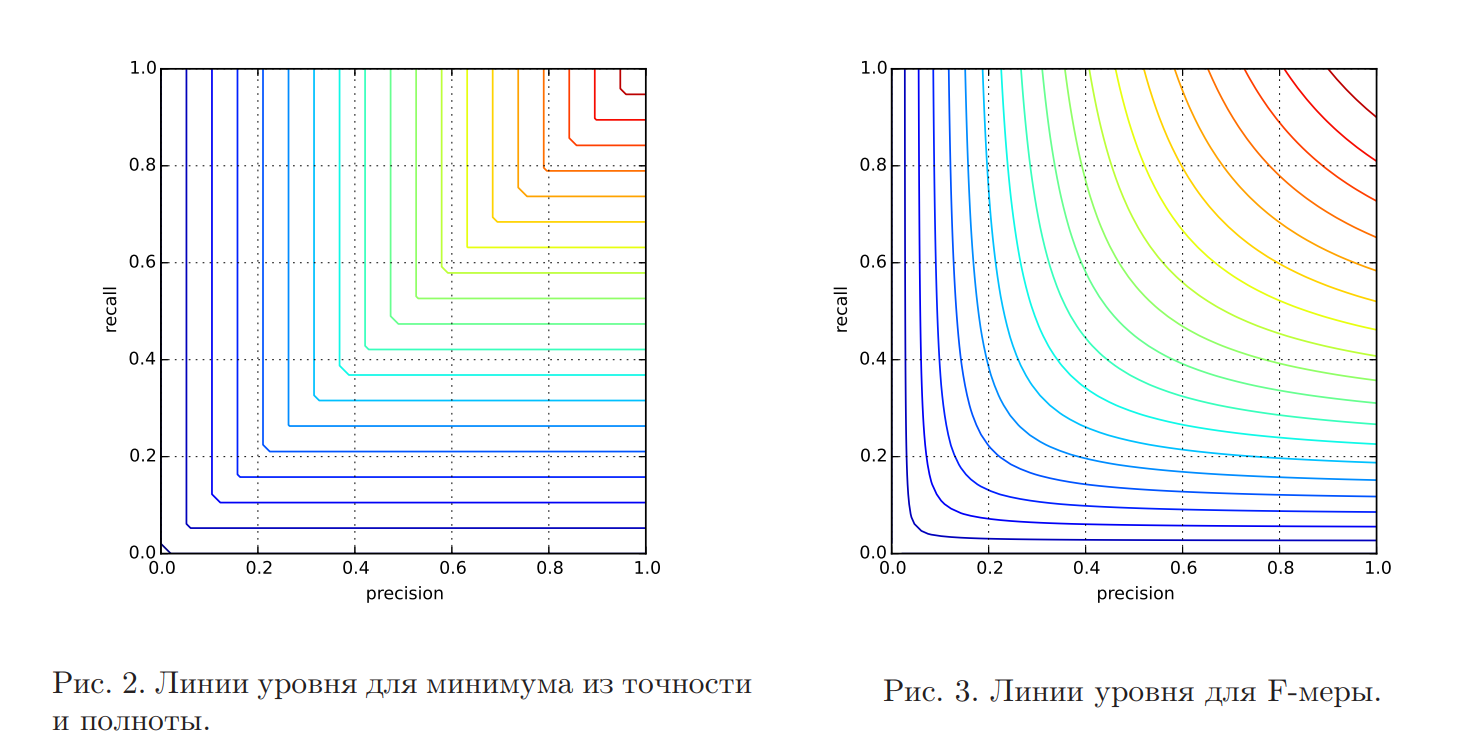
\includegraphics[width=18cm]{f-measure.png}

Кстати, есть ещё R-точность. Она равна точности при таком пороге $t$, при котором полнота равна точности:

\[ t* = argmin_t |precision(sign(b(x)-t)) - recall(sign(b(x) - t))| \]

\[R-precision = precision(sign(b(x)-t*))\]

То есть R-precision равна точности при таком пороге, при котором количество отнесённых к положительному классу объектор равно фактическому количеству положительных объектов в выборке.

Ещё есть lift. Есть задачи, связанные с выбором подмножества: выделение лояльных клиентов банка, обнаружение уходящих пользователей мобильного оператора и т.д. Заказчика может интересовать вопрос, насколько выгоднее работать с этим подмножеством по сравнению со всем множеством.
Интерпретируется lift как улучшение доли положительных объектов в подмножестве относительно доли в случайно выбранном подмножестве такого же размера.

\[ lift = \frac{precision}{\frac{TP+FN}{l}} \]

\item \textit{Для чего нужен порог в линейном классификаторе? Из каких соображений он может
выбираться?}

Порог нужен, чтобы определять баланс между precision и recall в зависимости от того, чего мы хотим добиться.
Может мы хотим минимизировать ложноположительные результаты или наоборот ложноотрицательные.

\item \textit{Что такое AUC-ROC? Опишите алгоритм построения ROC-кривой.}

AUC-ROC - метрика, равная площадью под кривой, которая вот как строится:

\[ FPR = \frac{FP}{FP+TN} \]

\[ TPR = \frac{TP}{TP+FN} \]

Отсортируем объекты по $\langle w, x \rangle$ и будем перебирать порог $t$ в $a(x) = sign(\langle w, x \rangle - t)$ и отмечать точки $(FPR, TPR)$.
AUC-ROC интерпретируется как вероятность того, что для случайно выбранных положительного объекта $x_+$ и отрицетельного $x_-$ будет выполнено $b(x_+) > b(x_-)$.

Кстати AUC-ROC тоже чувствителен к дисбалансу классов.


\item \textit{Что такое AUC-PRC? Опишите алгоритм построения PR-кривой.}

Идея та же, что и в AUC-ROC, только откладываем $(precision, recall)$. Только тут уже нет проблемы с несбалансированными классами.

\item \textit{. Что означает “модель оценивает вероятность положительного класса”? Как можно
внедрить это требование в процедуру обучения модели?}

Если говорят, что модель уверена в ответе на $95$ процентов, то если взять все объекты с $95$ процентов, то $95$ процентов из них будут положительными.

Классификатор $b$ верно оценивает вероятности, если при $P$ мы возьмём все $x \in \mathbb{X}$ с $b(x) = P$ и среди них доля положительных равна $P$.

Мы допускаем, что для одинакового признакового описания ответ будет разный. Причём если устремлять количество таких объектов в бесконечность, то доля положительных будет стремиться к $p(y=+1|x)$.

То есть хотим $argmin_{b \in \mathbb{R}} \frac{1}{n} \sum_{i=1}^n L(y_i, b) \approx p(y=+1|x)$

А если устремить $n \rightarrow +\infty$, то 
\[ argmin_{b \in \mathbb{R}} \mathbb{E} L(y, b) \approx p(y=+1|x) \]

\item \textit{Запишите функционал логистической регрессии. Как он связан с методом максимума
правдоподобия?}

\[ Q(a, X) =  \sum_{i=1}^l \log (1+\exp(-y_i \langle w, x_i \rangle )\]

Если наш алгоритм $b$ выдает вероятности, то вероятность того, что в выборке встретится $x_i$ с классом $y_i$ равна $b(x)^{[y+i = +1]}\cdot (1-b(x_i))^{[y_i=-1]}$

\[ Q(a, X) = \prod_{i=1}^l b(x)^{[y+i = +1]}\cdot (1-b(x_i))^{[y_i=-1]} \]

Логарифмируем:

\[ - \sum_{i=1}^l \left( [y+i = +1] \log b(x_i) + [y_i = -1] \log (1-b(x_i) \right) \rightarrow \min \]

Давайте преобразуем ответы $b$, чтобы он отдавал ответы в $[0,1]$:

\[ p(y=1|x) - \frac{1}{1+\exp(-\langle w, x \rangle)} \]

\[ Q(a, X) = - \sum_{i=1}^l \left( [y_i = +1] \log \frac{1}{1+\exp(-\langle w, x_i \rangle)} + [y_i = -1] \log \frac{\exp(-\langle w, x_i \rangle)}{1 + \exp(-\langle w, x_i \rangle)} \right) = \]

\[
= - \sum_{i=1}^l \left( [y_i = +1] \log \frac{1}{1+\exp(-\langle w, x_i \rangle)} + [y_i = -1] \log \frac{1}{1 + \exp(\langle w, x_i \rangle)} \right) = 
\]

\[ = \sum_{i=1}^l \log \left( 1+\exp(-y_i \langle w, x_i \rangle) \right) \]

\end{itemize}

\end{document}
